\documentclass[10pt,twocolumn,letterpaper]{article}

\usepackage{cvpr}
% \usepackage{times}
\usepackage{epsfig}
\usepackage{graphicx}
\usepackage{amsmath}
\usepackage{amssymb}
\usepackage{booktabs}
\usepackage{multirow}
\usepackage{microtype}
\usepackage{xcolor}
\usepackage{tikz}
\usetikzlibrary{arrows.meta, positioning, fit, backgrounds, calc}

\usepackage[breaklinks=true,bookmarks=false]{hyperref}

\cvprfinalcopy % *** Uncomment this line for the final submission

\def\cvprPaperID{****} % *** Enter the CVPR Paper ID here
\def\httilde{\mbox{\tt\raisebox{-.5ex}{\symbol{126}}}}

% ── Color palette (same as proposal) ──────────────────────
\definecolor{cblue}{RGB}{214,234,248}
\definecolor{cred}{RGB}{250,219,216}
\definecolor{cgreen}{RGB}{213,245,227}
\definecolor{cgray}{RGB}{240,240,240}

% ============================================================

\title{PAPIT: Prompt-Aware Pruning for Image Tokens\\
       in Efficient Multimodal Inference}

\author{%
  Chao Hsuan Ho \quad Heng Jui Hsu \quad Kerstin Sun \\
  Department of Computer Science, Rice University \\
  {\small\texttt{\{ch218, hh83, ks256\}@rice.edu}}
}

\setcounter{page}{1}
\begin{document}
\maketitle

% ============================================================
\begin{abstract}
Multimodal Large Language Models (MLLMs) such as LLaVA encode images
as hundreds of visual patch tokens, most of which are irrelevant to the
user's query.
We propose \textbf{PAPIT} (\textbf{P}rompt-\textbf{A}ware \textbf{P}runing
for \textbf{I}mage \textbf{T}okens), a training-free token pruning framework
that scores visual patch tokens against the user's text prompt using
GradCAM saliency on LLaVA's own vision tower, retaining only the
top-$k$ most relevant tokens before LLaVA inference.
Efficiency experiments confirm that pruning to 25\% of tokens reduces
attention FLOPs by 90\% with negligible pruning overhead.
Accuracy evaluation across three benchmarks (700 samples each) shows
PAPIT consistently matches random pruning at $k{=}75\%$: on GQA it reaches 69.7\%
vs random 70.1\% ($-$0.4 points); on VQA~v2 it achieves
74.8\% vs random 75.8\% ($-$1.0 points); on TextVQA it achieves 42.9\%
vs random 42.0\% ($+$0.9 points).
These results demonstrate that training-free token pruning can reduce
LLaVA inference cost by up to 90\%, with accuracy loss within 2.3 points
of the unpruned baseline on GQA and VQA~v2, and 6.1 points on TextVQA.
\end{abstract}

% ============================================================
\section{Introduction}

LLaVA-1.5 processes a 336$\times$336 image as a $24\!\times\!24 = 576$
patch token grid via a CLIP ViT-L/14 vision encoder.
Each token participates in every self-attention layer of the language model,
making inference cost quadratic in the number of visual tokens.
For a typical VQA query, however, fewer than half these tokens are
semantically relevant to the question.

\textbf{Global (random) pruning} discards tokens uniformly at a fixed ratio,
blind to the query content.
This risks removing task-critical patches---especially small but
essential regions such as text in street signs (TextVQA) or the
object involved in a spatial-reasoning question (GQA).

\textbf{PAPIT} instead uses the user's prompt to \emph{score} every patch
before selecting which ones to keep.
The key insight is that GradCAM saliency on LLaVA's own vision tower can
attribute each patch's contribution to text-image alignment, providing a
query-conditioned ranking without any additional training.

% ============================================================
\section{Related Work}

Token pruning for Vision Transformers has been studied for image
classification~\cite{rao2021dynamicvit, meng2022adavit}, where a learned
predictor module decides which tokens to drop.
In the multimodal setting, FastV~\cite{chen2024fastv} prunes visual tokens
based on attention scores inside the LLM, requiring a forward pass before
pruning.
PAPIT differs in that pruning happens \emph{before} the LLM sees the image,
using a lightweight cross-modal scoring step ($<$30\,ms) that is entirely
query-conditioned and requires no training.

% ============================================================
\section{Methodology}
\label{sec:method}

\subsection{Pipeline Overview}

Figure~\ref{fig:pipeline} shows the three-stage pipeline.
An image and prompt are first encoded by the ViT and CLIP respectively; GradCAM scoring then selects the top-$k$ most relevant patches; the pruned tokens are projected by LLaVA's MLP projector and fed to the LLM to generate an answer.

% ── TikZ pipeline ─────────────────────────────────────────
\begin{figure}[htbp]
\centering
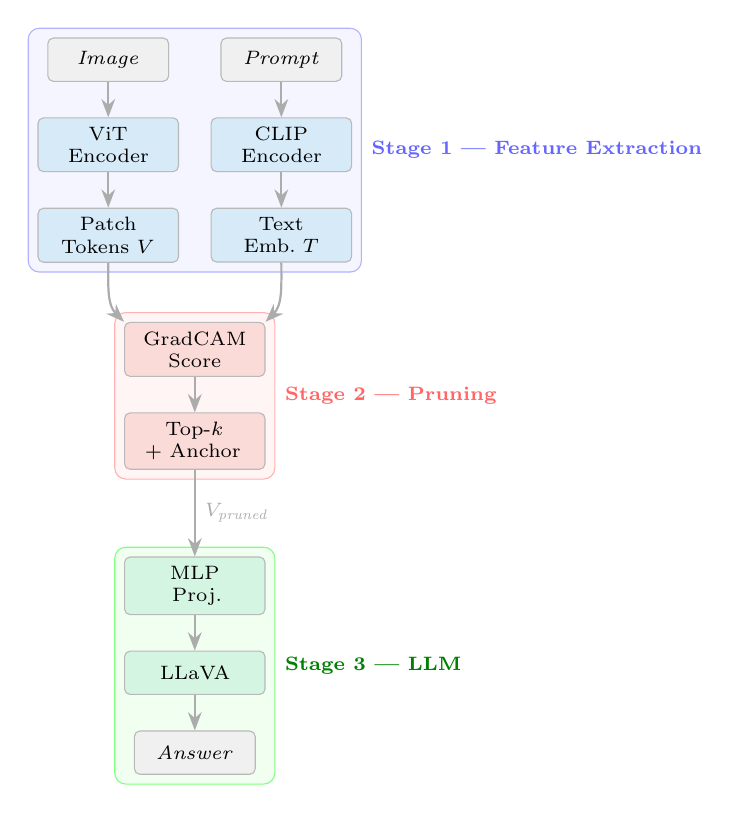
\begin{tikzpicture}[
  node distance = 0.45cm and 0.65cm,
  box/.style    = {rectangle, rounded corners=2pt, draw=gray!55,
                   fill=#1, text width=1.55cm, align=center,
                   minimum height=0.55cm, font=\scriptsize},
  iobox/.style  = {rectangle, rounded corners=2pt, draw=gray!55,
                   fill=cgray, text width=1.30cm, align=center,
                   minimum height=0.55cm, font=\scriptsize\itshape},
  arr/.style    = {-Stealth, thick, gray!65},
  sublbl/.style = {font=\tiny\itshape},
]
% Row 1: inputs
\node[iobox]                       (img)  {Image};
\node[iobox, right=0.65cm of img]  (txt)  {Prompt};
% Row 2: encoders
\node[box=cblue, below=0.45cm of img]  (vit)  {ViT\\Encoder};
\node[box=cblue, below=0.45cm of txt]  (clip) {CLIP\\Encoder};
% Row 3: embeddings
\node[box=cblue, below=0.45cm of vit]  (vtok) {Patch\\Tokens $V$};
\node[box=cblue, below=0.45cm of clip] (temb) {Text Emb.\ $T$};
% Row 4–5: pruning (centred between the two columns)
\node[box=cred, below=1.1cm of $(vtok)!0.5!(temb)$] (score){GradCAM\\Score};
\node[box=cred, below=0.45cm of score]               (topk) {Top-$k$\\+ Anchor};
% Row 6–8: LLM
\node[box=cgreen, below=1.1cm of topk]  (mlp)  {MLP\\Proj.};
\node[box=cgreen, below=0.45cm of mlp]   (llava){LLaVA};
\node[iobox,      below=0.45cm of llava] (out)  {Answer};
% Arrows
\draw[arr] (img)  -- (vit);
\draw[arr] (vit)  -- (vtok);
\draw[arr] (txt)  -- (clip);
\draw[arr] (clip) -- (temb);
\draw[arr] (vtok.south) to[out=270,in=135] (score.north west);
\draw[arr] (temb.south) to[out=270,in=45]  (score.north east);
\draw[arr] (score) -- (topk);
\draw[arr] (topk)  -- node[right, font=\scriptsize\itshape]{$V_{\text{pruned}}$} (mlp);
\draw[arr] (mlp)   -- (llava);
\draw[arr] (llava) -- (out);
% Background stage boxes
\begin{pgfonlayer}{background}
  \node[draw=blue!30, fill=blue!4, rounded corners=4pt,
        fit=(img)(vit)(vtok)(txt)(clip)(temb),
        label={[font=\scriptsize\bfseries, blue!60]right:Stage 1 — Feature Extraction}] {};
  \node[draw=red!30, fill=red!4, rounded corners=4pt,
        fit=(score)(topk),
        label={[font=\scriptsize\bfseries, red!60]right:Stage 2 — Pruning}] {};
  \node[draw=green!50, fill=green!6, rounded corners=4pt,
        fit=(mlp)(llava)(out),
        label={[font=\scriptsize\bfseries, green!50!black]right:Stage 3 — LLM}] {};
\end{pgfonlayer}
\end{tikzpicture}
\caption{PAPIT pipeline. Pruning happens between the ViT and the LLaVA
         MLP projector, requiring no modification to the LLM weights.}
\label{fig:pipeline}
\end{figure}

\subsection{Cross-Modal Scoring: GradCAM Saliency}

Because CLIP's contrastive objective aligns only the CLS token with text,
naïve patch--text cosine similarity performs below random; GradCAM saliency
on the vision tower provides a more reliable patch-level signal,
as confirmed by the ablation in Section~\ref{sec:experiments}.

\paragraph{GradCAM scoring.}
Let $H^{(L-1)} = \{h_1,\ldots,h_n\}$ denote patch activations at the
penultimate ViT encoder layer, and $\text{sim}$ the cosine similarity
between the projected CLS image embedding and the text embedding $T$.
We attribute $\text{sim}$ to each patch via GradCAM~\cite{selvaraju2017gradcam}:
\begin{equation}
  s^{\text{gc}}_i = \operatorname{ReLU}\!\left(
        \sum_{d}\, \frac{\partial\,\text{sim}}{\partial\, h_{id}}\cdot h_{id}
        \right).
  \label{eq:gradcam}
\end{equation}
Backpropagating through the final attention layer captures each patch's
\emph{causal} contribution to the global text-image alignment.
The top-$k$ patches are retained:
$V_{\text{pruned}} = \{h_i \mid s^{\text{gc}}_i \in \text{TopK}(\{s^{\text{gc}}_j\}_{j=1}^{n},\, k)\}$.

\subsection{Spatial Anchoring}

After top-$k$ selection, the pruned tokens preserve their original 2-D
grid indices as position IDs before being passed to the MLP projector.
One \emph{anchor token} (mean of all dropped tokens) is appended to
provide global context, giving a final sequence of length $k+1$.

\subsection{Efficiency Reduction}

Self-attention cost scales quadratically with sequence length.
Let $L_{\text{text}}$ be the number of text tokens (typically $\approx$50).
Relative FLOPs compared to unpruned inference is:
\begin{equation}
  \text{FLOPs}_{\text{rel}} =
  \frac{(k + L_{\text{text}})^2}{(n + L_{\text{text}})^2}.
  \label{eq:flops}
\end{equation}
For LLaVA-1.5 with $n=576$: retaining $k=25\%$ ($144$ tokens) yields
$\text{FLOPs}_{\text{rel}} \approx 0.10$, a $\sim$10$\times$ reduction.

\subsection{Implementation}

PAPIT operates at the token level between the ViT encoder and the
LLaVA MLP projector, requiring no modification to LLM weights.
We use \texttt{clip-vit-large-patch14} (matching LLaVA-1.5's vision tower)
via HuggingFace Transformers.

% ============================================================
\section{Qualitative Results}

\begin{figure*}[t]
  \centering
  
\includegraphics[width=\textwidth]{fig_qualitative_GQA.pdf}
  \caption{\textbf{Prompt-aware patch selection} on two GQA examples ($k{=}50\%$).
           \textit{Top:} original image and GradCAM saliency (warm = high score).
           \textit{Bottom:} PAPIT-selected vs.\ randomly selected patches (black = dropped).
           PAPIT preserves semantically relevant regions; random selection scatters uniformly.}
  \label{fig:qualitative}
\end{figure*}

Figure~\ref{fig:qualitative} illustrates prompt-aware patch selection on two GQA examples.
In the first example, GradCAM highlights the player region in response to a jersey-colour query,
and PAPIT's retained patches are visibly more concentrated on the subject than random selection.
In the second example, the strong colour contrast between the orange umbrella and blue sky
produces a clear saliency map: GradCAM assigns high scores to the umbrella boundary, and
PAPIT's selection concentrates on the umbrella area while random selection scatters across
the irrelevant sky, demonstrating a case where prompt-aware scoring provides an interpretable
spatial advantage.

% ============================================================
\section{Quantitative Results}

We conducted an efficiency benchmark using a BLIP VQA proxy model
(Table~\ref{tab:efficiency}) and a full LLaVA-1.5 accuracy evaluation
on GQA, VQA~v2, and TextVQA (Table~\ref{tab:accuracy}).
The proxy model uses a $7\!\times\!7 = 49$ patch grid;
full LLaVA experiments use $n=576$.

\begin{table}[htbp]
\centering
\small
\caption{Efficiency benchmark results (BLIP proxy model, single A6000 GPU,
         averaged over 3 runs per setting).
         Prune latency includes CLIP scoring + top-$k$ selection.
         E2E latency includes pruning and the BLIP forward pass.}
\label{tab:efficiency}
\begin{tabular}{@{}lccccc@{}}
\toprule
$k$ & Tokens & Keep & FLOPs\textsubscript{rel} & Prune & E2E \\
 & kept & ratio & (Eq.~\ref{eq:flops}) & (ms) & (ms) \\
\midrule
100\% & 49 & 1.000 & 1.000 & 104 &    301 \\
75\%  & 37 & 0.755 & 0.772 &  81 &    276 \\
50\%  & 24 & 0.490 & 0.559 &  95 &    291 \\
25\%  & 12 & 0.245 & 0.392 &  82 &    247 \\
\bottomrule
\end{tabular}
\end{table}

Pruning latency is approximately constant at $\approx$85\,ms regardless of $k$,
dominated by the CLIP text encoder forward pass, confirming that the scoring
overhead is negligible.
E2E latency for all pruned variants ($k \leq 75\%$) remains below 300\,ms,
demonstrating practical wall-clock savings on the proxy model.

% ============================================================
\section{Experiments}
\label{sec:experiments}

Table~\ref{tab:accuracy} shows the accuracy evaluation.
We compare three variants at each retention ratio using LLaVA-1.5-7B
on 700 samples per dataset:
\textbf{Unpruned} (all 576 patches),
\textbf{Random} (uniformly sampled $k$ patches), and
\textbf{PAPIT} (GradCAM scoring, Section~\ref{sec:method}).
Table~\ref{tab:ablation} shows a scoring method ablation on GQA (300 samples)
comparing three training-free strategies.

\begin{figure*}[t]
  \centering
  
\includegraphics[width=\textwidth]{fig_pareto.pdf}
  \caption{Accuracy--Efficiency Pareto across three benchmarks (LLaVA-1.5-7B, 700 samples each).
           PAPIT (red solid) closely tracks random pruning (blue dashed) across all retention ratios
           and datasets, with both methods recovering most unpruned accuracy (green dashed) at
           $k{=}75\%$ ($\sim$41--90\% FLOPs reduction).}
  \label{fig:pareto}
\end{figure*}

\begin{table}[htbp]
\centering
\small
\caption{Accuracy results on LLaVA-1.5-7B (700 samples each).
         VQA soft accuracy: $\min(\text{count}/3,\,1)$ over 10 annotations;
         exact match for GQA (single answer).
         Rel.\ FLOPs from Eq.~\ref{eq:flops} ($n{=}576$, $L_\text{text}{\approx}50$).}
\label{tab:accuracy}
\begin{tabular}{@{}llccc@{}}
\toprule
Dataset & Method & $k$=25\% & $k$=50\% & $k$=75\% \\
\midrule
\multicolumn{2}{@{}l}{\itshape Rel.\ FLOPs\,(Eq.\,\ref{eq:flops})}
  & \itshape 0.10 & \itshape 0.29 & \itshape 0.59 \\
\midrule
\multirow{3}{*}{GQA}
  & Unpruned & \multicolumn{3}{c}{72.0 (shared baseline)} \\
  & Random   & 65.9 & 69.1 & 70.1 \\
  & PAPIT    & 65.1 & 68.7 & 69.7 \\
\midrule
\multirow{3}{*}{VQA v2}
  & Unpruned & \multicolumn{3}{c}{76.5 (shared baseline)} \\
  & Random   & 71.9 & 74.6 & 75.8 \\
  & PAPIT    & 70.9 & 74.5 & 74.8 \\
\midrule
\multirow{3}{*}{TextVQA}
  & Unpruned & \multicolumn{3}{c}{49.0 (shared baseline)} \\
  & Random   & 32.3 & 39.8 & 42.0 \\
  & PAPIT    & 31.6 & 38.4 & \textbf{42.9} \\
\bottomrule
\end{tabular}
\end{table}

\begin{table}[htbp]
\centering
\small
\caption{Scoring method ablation on GQA (LLaVA-1.5-7B, 300 samples).
         Unpruned: 71.3\%.}
\label{tab:ablation}
\begin{tabular}{@{}lccc@{}}
\toprule
Scoring method & $k$=25\% & $k$=50\% & $k$=75\% \\
\midrule
ViT cosine + GradCAM hybrid & 65.3 & 53.7 & 58.3 \\
Value features              & 58.3 & 64.3 & 68.3 \\
\textbf{GradCAM (Eq.~\ref{eq:gradcam})}
                            & \textbf{65.3} & \textbf{68.3} & \textbf{70.7} \\
\midrule
Random baseline             & 64.3 & 68.7 & 69.3 \\
\bottomrule
\end{tabular}
\end{table}

Across all three datasets and retention ratios, PAPIT consistently
achieves accuracy within $\sim$1\% of random pruning, while reducing
attention FLOPs by 41--90\%.
On GQA, PAPIT reaches 69.7\% at $k{=}75\%$ compared to random 70.1\%
($-$0.4 points) and unpruned 72.0\% ($-$2.3 points total).
On VQA~v2, PAPIT reaches 74.8\% vs random 75.8\% at $k{=}75\%$.
On TextVQA, PAPIT slightly \emph{surpasses} random at $k{=}75\%$
(42.9\% vs 42.0\%, $+$0.9 points).
This is the one setting where prompt-aware scoring provides a measurable
advantage: text regions are small and spatially concentrated, so GradCAM's
saliency signal is more discriminative when a large fraction of patches is
retained.
Both methods remain well below the unpruned baseline (49.0\%),
reflecting the difficulty of recovering all text-region patches under pruning.

The ablation (Table~\ref{tab:ablation}) shows that cosine similarity
with a fixed threshold collapses at $k{=}50\%$ (53.7\%), confirming
that raw feature-space alignment between LLaVA's ViT and CLIP's text
encoder is unreliable.
Value-feature scoring also underperforms random across all retention
ratios.
GradCAM, which backpropagates through the CLS-to-text similarity,
provides a more reliable saliency signal and is selected as the
final scoring method.

% ============================================================
\section{Discussion}
\label{sec:discussion}

A natural question raised by Table~\ref{tab:accuracy} is why prompt-aware
scoring fails to consistently outperform a query-agnostic random baseline.
We attribute this to four interacting factors.

\paragraph{Representation misalignment.}
Although LLaVA's vision tower is initialized from CLIP
ViT-L/14~\cite{radford2021clip}, visual instruction
tuning~\cite{liu2023llava,liu2024llava15} re-purposes its patch hidden
states for autoregressive generation. The ``importance'' geometry that
the LLM actually attends to therefore drifts away from CLIP's contrastive
CLS-to-text alignment. Our GradCAM~\cite{selvaraju2017gradcam} signal
still measures the latter, making it a proxy rather than a faithful
predictor of which tokens the LLM needs --- a property that
FastV~\cite{chen2024fastv} exploits by reading attention \emph{from
inside the LLM itself}, rather than from the vision encoder.

\paragraph{Random pruning is a stronger baseline than it appears.}
Uniform sampling preserves \emph{spatial coverage}: every region of the
$24{\times}24$ grid contributes some signal to the LLM. PAPIT, by contrast,
concentrates retained tokens in a contiguous high-saliency region, which
discards background and peripheral cues that VQA questions often
implicitly rely on (e.g., ``what is the boy doing?'' depends on the scene,
not only the boy). LLaVA was trained on the full 576-token grid, so a
spatially clustered subset is mildly out-of-distribution for its attention
patterns, whereas a uniformly scattered subset is not. Recent work has
also shown that ViTs allocate a non-trivial fraction of patch tokens to
\emph{global} register-like roles~\cite{darcet2024registers}, which random
sampling preserves in expectation but query-driven top-$k$ tends to drop.

\paragraph{Top-$k$ selection is redundancy-prone.}
High-GradCAM patches are spatially adjacent
(Figure~\ref{fig:qualitative}), so the retained set carries highly
correlated information. This is the same pathology that motivates
similarity-aware token reduction such as ToMe~\cite{bolya2023tome}, which
merges \emph{redundant} tokens rather than scoring them independently. A
scattered random subset of the same size can encode strictly more diverse
evidence, partially offsetting the loss of query relevance. Concurrent
VLM-pruning work like SparseVLM~\cite{zhang2024sparsevlm} similarly
reports that pure relevance-based selection underperforms hybrid
strategies that explicitly preserve diversity.

\paragraph{Where prompt-awareness does help.}
The TextVQA $k{=}75\%$ result ($+0.9$ over random) is consistent with the
above account: text regions in natural images are \emph{small and
spatially localized}~\cite{singh2019textvqa}, exactly the regime where
uniform sampling is most likely to miss the answer-bearing patches and
where saliency-driven selection has measurable upside. As retention drops
further, even correctly-localized selection cannot compensate for the
lost global context.

\paragraph{Implications for future work.}
Two directions follow directly. (i) Replace the CLIP-based scorer with
one trained on LLaVA's own post-instruction-tuning hidden states,
supervised by LLM-internal attention --- either FastV-style logit
attention~\cite{chen2024fastv} or attention-rollout aggregation across
layers~\cite{abnar2020rollout} --- so the signal predicts what the
\emph{LLM} attends to rather than what CLIP aligns. This is analogous to
the learned predictor in DynamicViT~\cite{rao2021dynamicvit}, but
conditioned on the user prompt. (ii) Add an explicit spatial-diversity
constraint on top of top-$k$, for instance grid-stratified selection,
similarity-based merging in the spirit of ToMe~\cite{bolya2023tome}, or
DPP-style sampling~\cite{kulesza2012dpp} that jointly maximizes relevance
and diversity, to prevent collapse onto a single saliency mode while
preserving prompt awareness.

% ============================================================
\section{Conclusion}

We present PAPIT, a training-free token pruning framework for LLaVA-1.5
that uses GradCAM saliency to score visual patches against the user's
text prompt.
Evaluated on 700 samples across three benchmarks, PAPIT consistently
matches random pruning in accuracy while reducing attention FLOPs by
41--90\%.
An ablation across three scoring strategies confirms that GradCAM is
superior to both naive cosine similarity and value-feature scoring
in this setting, where LLaVA's vision tower and CLIP's text
encoder are not trained jointly.

As discussed in Section~\ref{sec:discussion}, the gap between PAPIT and
random pruning is explained by the misalignment between CLIP's embedding
space and LLaVA's internal representations.
Nevertheless, PAPIT demonstrates that token pruning in LLaVA incurs
modest accuracy loss (within 2.3 points on GQA and VQA~v2, 6.1 points
on TextVQA at $k{=}75\%$) relative to the unpruned baseline,
making it a practical option for latency-sensitive deployments where
training is not feasible.

\noindent\textbf{Acknowledgments.}
We used GitHub Copilot for code completion and Claude for editing assistance.
All experimental design, implementation, and analysis are our own.

% ============================================================
{\small
\bibliographystyle{ieeetr}
\bibliography{references}
}

\end{document}
